\section{Auswertung}
	\label{sec:auswertung}
	\begin{table}
\begin{center}
\begin{tabular}{r|r|r|r|r|r|r|r}
f[$\SI{}{\kilo\hertz}$] & U[$\SI{}{\volt}$] & f[$\SI{}{\kilo\hertz}$] & U[$\SI{}{\volt}$] & f[$\SI{}{\kilo\hertz}$] & U[$\SI{}{\volt}$] & f[$\SI{}{\kilo\hertz}$] & U[$\SI{}{\volt}$] \\
\hline
1 & 2.6 & 29 & 7.4 & 32.8 & 9.9 & 33.7 & 10 \\
5 & 2.6 & 30 & 8.2 & 33 & 10 & 33.8 & 9.9 \\
10 & 2.8 & 30.5 & 8.6 & 33.1 & 10 & 33.9 & 9.9 \\
15 & 3.2 & 31 & 9 & 33.2 & 10 & 34 & 9.9 \\
20 & 3.9 & 31.5 & 9.3 & 33.23 & 10 & 34.2 & 9.8 \\
25 & 5.2 & 32 & 9.6 & 33.3 & 10 & 34.4 & 9.7 \\
26 & 5.7 & 32.2 & 9.7 & 33.4 & 10 & 34.6 & 9.6 \\
27 & 6.2 & 32.4 & 9.8 & 33.5 & 10 & 34.8 & 9.5 \\
28 & 6.8 & 32.6 & 9.9 & 33.6 & 10 & 35 & 9.3 \\
\end{tabular}
\end{center}
\begin{center}
\begin{tabular}{r|r|r|r|r|r}
f[$\SI{}{\kilo\hertz}$] & U[$\SI{}{\volt}$] & f[$\SI{}{\kilo\hertz}$] & U[$\SI{}{\volt}$] & f[$\SI{}{\kilo\hertz}$] & U[$\SI{}{\volt}$] \\
\hline
35.2 & 9.2 & 39 & 5.9 & 60 & 1.1 \\
35.4 & 9 & 39.5 & 5.5 & 65 & 0.9 \\
35.6 & 8.8 & 40 & 5.2 & 70 & 0.7 \\
35.8 & 8.7 & 41 & 4.6 & 80 & 0.5 \\
36 & 8.5 & 42 & 4.1 & 90 & 0.4 \\
36.5 & 8 & 43 & 3.7 & 100 & 0.3 \\
37 & 7.5 & 44 & 3.4 & 125 & 0.1 \\
37.5 & 7.1 & 45 & 3.1 & 150 & 0.1 \\
38 & 6.7 & 50 & 2.0 & 200 & 0 \\
38.5 & 6.3 & 55 & 1.5 \\
\end{tabular}
\caption[Messwerte zu Aufgabenteil c]{Frequenzabh"angigkeit der Kondensatorspannung an einem Serienresonanzkreis}
\label{frequenz}
\end{center}
\end{table}


	\subsection{Zeitabh"angigkeit der Amplitude eines ged"ampften Schwingung} % (fold)
	\label{sub:zeitabh"angigkeit_der_amplitude_eines_ged"ampften_schwingung}
	
	Die Zeitabh"angigkeit der Amplitude einer ged"ampften Schwingung ist in Graph \eqref{amplitude} zu sehen.
	Aus dem Graphen \eqref{amplitude} wurden die Amplituden aus Tabelle \eqref{amplitude} entnommen. Mit einer linearen Ausgleichsrechnung der logarithmierten  Amplituden mit Gnuplot ergaben sich der Graph \eqref{amplitude_fit}. Die Ausgleichsrechnung f"uhrte auf die Werte:

	\begin{eqnarray}
		f(x) &=& -m \cdot x + b\\ \label{ausgleich}
		m &=& \SI{0.195 (3)}{1\per\centi\meter} \nonumber\\
		b &=& \SI{1.692 (11)}{\centi\meter}\nonumber 
	\end{eqnarray}

	Aus der Graphik wurde zur Bestimmung des Exponenten in $cm$ abgelesen.
	Dabei gilt: $\SI{1.55}{\centi\meter}\, \widehat{=} \,\SI{50}{\micro\second}$.
	Damit ergibt sich f"ur den Vorfaktor des Expontenen $2 \cdot \pi \cdot \mu$ der e-Funktion: 
	\begin{eqnarray*}
		\SI{1}{1\per\centi\meter} &\widehat{=}& \SI{0.031}{1\per\micro\second}\\
		2\cdot \pi \cdot \mu  = 0.031 \cdot m &=&  \SI{6.045 (93)}{\kilo \hertz}
	\end{eqnarray*}

	Daraus Folgt f"ur die Abklingdauer und den effektiven D"ampfungswiderstand:

	\begin{eqnarray*}
		L &=& \SI{10.14 (3)}{\milli \henry }\\
		\Rightarrow T_\mathrm{ex} &=& \frac{1}{2 \cdot \pi \cdot \mu} = \SI{0.16 (1)}{\milli \second}\\
		\Rightarrow R_\mathrm{eff} &=& 2 \cdot L \cdot 2 \cdot \pi \cdot \mu = \SI{122.59 (192)}{\ohm}
	\end{eqnarray*}
	\newpage

	Der Fehler von $R_\mathrm{eff}$ berechnet sich mit:

	\begin{eqnarray*}
		\Delta R_\mathrm{eff} &=& \sqrt{ \left( |\frac{\partial R}{\partial 2 \cdot \pi \cdot \mu}| \cdot \Delta 2 \cdot \pi \cdot \mu \right)^2 + \left( |\frac{\partial R}{\partial L}| \cdot \Delta L \right)^2}\\ \label{fehler}
		\Delta 2 \cdot \pi \cdot \mu &=& 93\\
		\Delta L &=& 0.00003\\
		\Rightarrow \Delta R_\mathrm{eff} &=& 1.92
	\end{eqnarray*}

	Der effektive D"ampfungswiderstand von $\SI{122.59 (192)}{\ohm}$ ist gr"o"ser als der verbaute Widerstand $R_\mathrm{eff,theo} = \SI{103.7 (1)}{\ohm}$. Dies l"asst sich durch die zus"atzlichen Ohm'schen Widest"ande in der Spule und den Leitungen erkl"aren.

	\clearpage

	\begin{figure}[H]
		\centering
		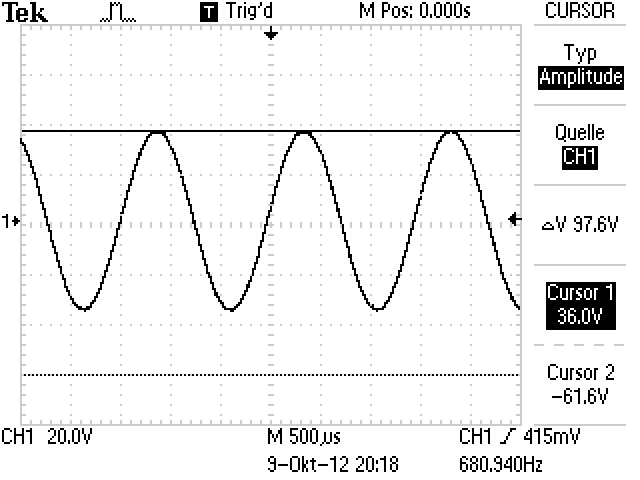
\includegraphics[width = 12cm]{img/F0006TEK.jpg}
		\caption{Zeitabh"angigkeit der Amplitude einer ged"ampften Schwingung. Mit rot ist die Einh"ullende gekennzeichnet.}
		\label{amplitude}
	\end{figure}

	\begin{figure}[H]
		\centering
		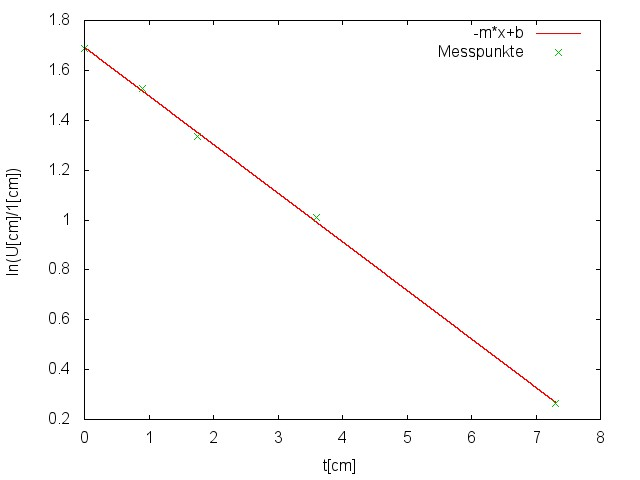
\includegraphics[width = 12cm]{img/graph_a_2.jpg}
		\caption{Amplituden aus Graph \eqref{amplitude} mit einer Ausgleichsrechnung mittels \eqref{ausgleich}}
		\label{amplitude_fit}
	\end{figure}

	\begin{table}[!h]
\begin{center}
\begin{tabular}{|r|r|r|r|}
\hline
f[$\SI{}{\kilo\hertz}$] & U[$\SI{}{\milli\volt}$] & f[$\SI{}{\kilo\hertz}$] & U[$\SI{}{\milli\volt}$]\\
\hline
\hline
25.0 &	0.0 &	35.1 &	6.1 \\	
30.0 &	0.2 &	35.2 &	4.9 \\	
30.5 &	0.2 &	35.3 &	4.0 \\	
31.0 &	0.3 &	35.4 &	3.4 \\	
31.5 &	0.4 &	35.5 &	2.9 \\	
32.0 &	0.5 &	35.6 &	2.5 \\	
32.5 &	0.6 &	35.7 &	2.2 \\	
33.0 &	0.7 &	35.8 &	2.0 \\	
33.5 &	1.1 &	35.9 &	1.8 \\	
34.0 &	1.8 &	36.0 &	1.6 \\	
34.1 &	2.0 &	36.5 &	1.1 \\	
34.2 &	2.3 &	37.0 &	0.8 \\	
34.3 &	2.7 &	37.5 &	0.6 \\	
34.4 &	3.1 &	38.0 &	0.5 \\	
34.5 &	3.8 &	38.5 &	0.4 \\	
34.6 &	4.6 &	39.0 &	0.3 \\	
34.7 &	5.9 &	39.5 &	0.3 \\	
34.8 &	7.4 &	40.0 &	0.2 \\	
34.9 &	8.6 &	40.5 &	0.0 \\	
35.0 &	7.4 &  & \\
\hline
\end{tabular}
\end{center}

	\subsection{Bestimmung des D"ampfungswiderstands $R_\mathrm{ap}$} % (fold)
	\label{sub:bestimmung_des_d_ampfungswiderstands_r_}
	

	F"ur die Suche nach dem aperiodischen Grenzfall ergaben sich die Graphiken \eqref{ap_1} bis \eqref{ap_3}.
	Dabei zeigt Graphik \eqref{ap_2} den aperiodischen Grenzfall bei etwa :

	\begin{equation*}
		R_\mathrm{ap} = \SI{3.52}{\kilo\ohm}.
	\end{equation*}
		F"ur den errechneten Wert ergab sich :
	\begin{eqnarray*}
		C &=& \SI{2.088 (6)}{\nano \farad}\\
		L &=& \SI{10.14 (3)}{\milli \henry}\\
		R_\mathrm{ap} = \sqrt{\frac{4 \cdot L}{C}} &=& \SI{3.12 (652)}{\kilo\ohm}.
	\end{eqnarray*}

	Dies entspricht einer Abweichung von etwa $\SI{13}{\%}$.
	Der Fehler berechnet sich nach:

	\begin{equation}
		\Delta R_\mathrm{ap} = \sqrt{ \left( |\frac{\partial R}{\partial C}| \cdot \Delta C \right)^2 + \left( |\frac{\partial R}{\partial L}| \cdot \Delta L \right)^2}
	\end{equation}
\clearpage
	\begin{figure}[H]
			\centering
			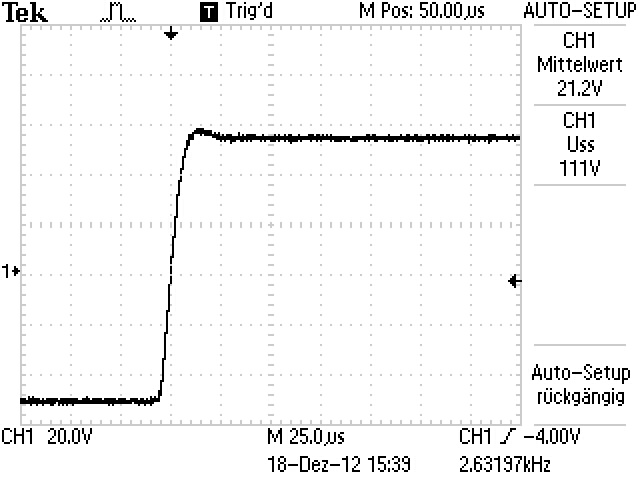
\includegraphics[width = 12cm]{img/F0003TEK.jpg}
			\caption{"Uberd"ampfung}
			\label{ap_1}
		\end{figure}	

		\begin{figure}[H]
			\centering
			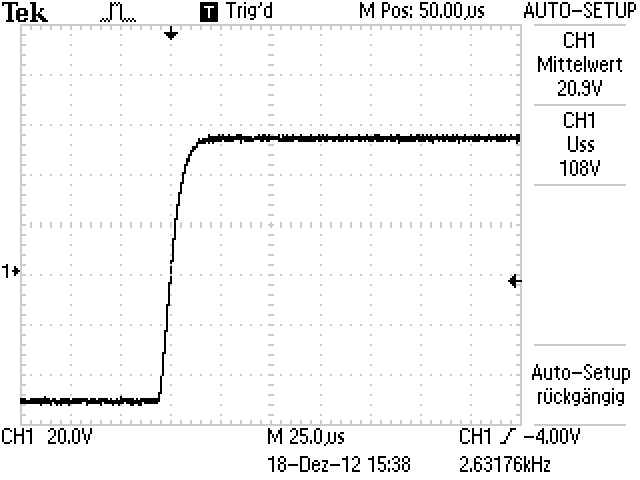
\includegraphics[width = 12cm]{img/F0002TEK.jpg}
			\caption{Aperiodischer Grenzfall}
			\label{ap_2}
		\end{figure}

	\begin{figure}[H]
		\centering
		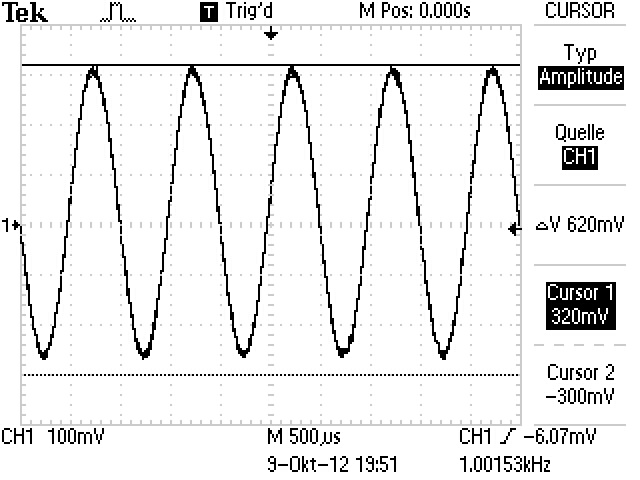
\includegraphics[width = 12cm]{img/F0001TEK.jpg}
		\caption{Kriechfall}
		\label{ap_3}
	\end{figure}

	\subsection{Frequenzabh"angigkeit der Kondensatorspannung} % (fold)
	\label{sub:frequenzabh"angigkeit_der_kondensatorspannung}
	
	Bei der Messung der frequenzabh"angigkeit der Spannung ergaben sich die Werte aus Tabelle \eqref{frequenz}.
	Diese sind zudem in Graph \eqref{frequenz_1} dargestellt, wobei $U_\mathrm{c}$ mit $U_\mathrm{0} = \SI{2.6 (1)}{\volt}$ normiert wurde.
	Der Bereich um die Resonanzfrequenz ist in Graph \eqref{frequenz_2} dargestellt. Die Schnittpunkte des Graphen mit der Linie stellt dabei die Breite der Resonanzkurve dar.
	Bei diesem Versuch wurde der Gesamtwiderstand benutzt:

	\begin{eqnarray*}
		R_\mathrm{2} &=& \SI{523.9 (5)}{\ohm}\\
		R_\mathrm{i} &=& \SI{50}{\ohm}\\
		R_\mathrm{ges} &=& \SI{573.9 (5)}{\ohm}
	\end{eqnarray*}

	Das Maximum der Kurve gibt die Resonanz"uberh"ohung $q$ an, die Schnittpunkte $f_1$ und $f_2$ die Grenzen f"ur die Breite.
	Ablesen der Werte ergibt ungef"ahr:

	\begin{eqnarray*}
		q &=& \SI{3.846 (50)}{}\\
		f_1 &=& \SI{37.5 (5)}{\kilo\hertz}\\
		f_2 &=& \SI{28.5 (5)}{\kilo\hertz}\\
		\Rightarrow w_1 - w_2 = 2 \cdot \pi \cdot (f_1 - f_2) &=& \SI{56548.66 (1)}{\kilo\hertz}\\
	\end{eqnarray*}

	Dieser Wert liegt sehr nah an dem Referenzwert $R/L = \SI{56597.63 (279)}{\ohm \per \henry}$.
	Der errechnete Wert f"ur $q = \SI{3.840 (136)}{}$ weicht damit um nur etwa $\SI{0.2}{\%}$ vom abgelesenen Wert ab.
	Der Fehler errechnet sich vom Typ wie in Gleichung \eqref{fehler}.

	\begin{table}
\begin{center}
\begin{tabular}{r|r|r|r|r|r|r|r}
f[$\SI{}{\kilo\hertz}$] & U[$\SI{}{\volt}$] & f[$\SI{}{\kilo\hertz}$] & U[$\SI{}{\volt}$] & f[$\SI{}{\kilo\hertz}$] & U[$\SI{}{\volt}$] & f[$\SI{}{\kilo\hertz}$] & U[$\SI{}{\volt}$] \\
\hline
1 & 2.6 & 29 & 7.4 & 32.8 & 9.9 & 33.7 & 10 \\
5 & 2.6 & 30 & 8.2 & 33 & 10 & 33.8 & 9.9 \\
10 & 2.8 & 30.5 & 8.6 & 33.1 & 10 & 33.9 & 9.9 \\
15 & 3.2 & 31 & 9 & 33.2 & 10 & 34 & 9.9 \\
20 & 3.9 & 31.5 & 9.3 & 33.23 & 10 & 34.2 & 9.8 \\
25 & 5.2 & 32 & 9.6 & 33.3 & 10 & 34.4 & 9.7 \\
26 & 5.7 & 32.2 & 9.7 & 33.4 & 10 & 34.6 & 9.6 \\
27 & 6.2 & 32.4 & 9.8 & 33.5 & 10 & 34.8 & 9.5 \\
28 & 6.8 & 32.6 & 9.9 & 33.6 & 10 & 35 & 9.3 \\
\end{tabular}
\end{center}
\begin{center}
\begin{tabular}{r|r|r|r|r|r}
f[$\SI{}{\kilo\hertz}$] & U[$\SI{}{\volt}$] & f[$\SI{}{\kilo\hertz}$] & U[$\SI{}{\volt}$] & f[$\SI{}{\kilo\hertz}$] & U[$\SI{}{\volt}$] \\
\hline
35.2 & 9.2 & 39 & 5.9 & 60 & 1.1 \\
35.4 & 9 & 39.5 & 5.5 & 65 & 0.9 \\
35.6 & 8.8 & 40 & 5.2 & 70 & 0.7 \\
35.8 & 8.7 & 41 & 4.6 & 80 & 0.5 \\
36 & 8.5 & 42 & 4.1 & 90 & 0.4 \\
36.5 & 8 & 43 & 3.7 & 100 & 0.3 \\
37 & 7.5 & 44 & 3.4 & 125 & 0.1 \\
37.5 & 7.1 & 45 & 3.1 & 150 & 0.1 \\
38 & 6.7 & 50 & 2.0 & 200 & 0 \\
38.5 & 6.3 & 55 & 1.5 \\
\end{tabular}
\caption[Messwerte zu Aufgabenteil c]{Frequenzabh"angigkeit der Kondensatorspannung an einem Serienresonanzkreis}
\label{frequenz}
\end{center}
\end{table}


\clearpage

	\begin{figure}[H]
		\centering
		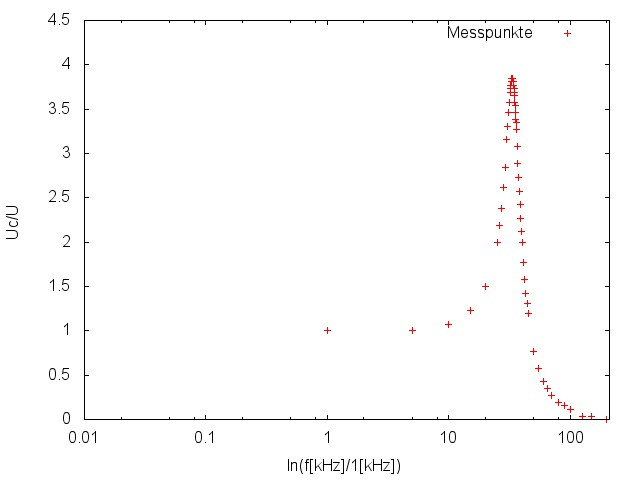
\includegraphics[width = 12cm]{img/graph_c.jpg}
		\caption{Frequenzabh"angigeit der Spannung}
		\label{frequenz_1}
	\end{figure}

	\begin{figure}[H]
		\centering
		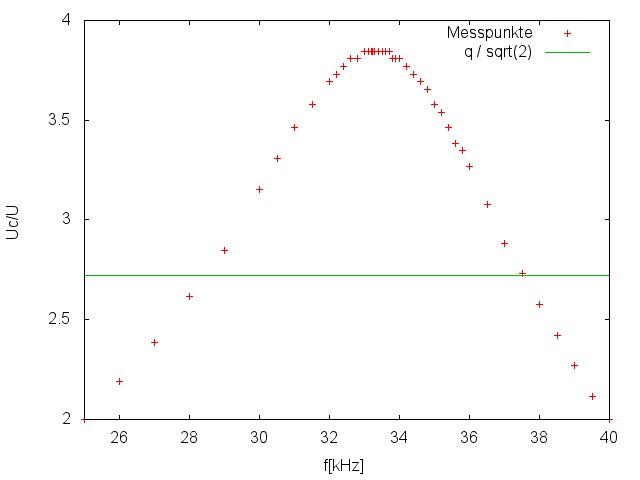
\includegraphics[width = 12cm]{img/graph_c_1.jpg}
		\caption{Frequenzabh"angigkeit der Spannung im Bereich um die Resonanzfrequenz}
		\label{frequenz_2}
	\end{figure}

	\subsection{Frequenzabh"angigkeit der Phase} % (fold)
	\label{sub:frequenzabh"angigkeit_der_phase}
	
	Die Messdaten zur Frequenzabh"angigkeit der Phasenverschiebung sind in Tabelle \eqref{phase} dargstellt.
	Der dazugeh"orige Graph \eqref{phase} zeigt die Messwerte und die signifikanten stellen bei $\Phi = 45^\circ$, $\Phi = 90^\circ$ und $\Phi = 135^\circ$.
	Diese entsprechen den Punkten, wo die Frequenz die Werte $f_2$, $f_\mathrm{res}$ und $f_1$ annimmt.

	Es ergibt sich f"ur die abgelesenen Werte:

	\begin{eqnarray*}
		w_2 = 2 \cdot \pi \cdot f_2 &=& \SI{188.496 (3142)}{\kilo \hertz}\\
		w_\mathrm{res} = 2 \cdot \pi \cdot f_\mathrm{res} &=& \SI{210.487 (3142)}{\kilo \hertz}\\
		w_1 = 2 \cdot \pi \cdot f_1 &=& \SI{241.903 (3142)}{\kilo \hertz}
	\end{eqnarray*}

	Die errechneten Werte ergeben:

	\begin{eqnarray*}
		w_1 = \frac{R}{2L} + \sqrt{\frac{R^2}{4\,L^2} + \frac{1}{L \, C}} &=& \SI{247.461 (414)}{\kilo \hertz}\\
		w_\mathrm{res} = \sqrt{\frac{1}{L\, C} - \frac{R^2}{2 \, L^2}} &=& \SI{217.290 (440)}{\kilo \hertz}\\
		w_2 = -\frac{R}{2L} + \sqrt{\frac{R^2}{4\,L^2} + \frac{1}{L \, C}} &=& \SI{190.863 (395)}{\kilo \hertz}
	\end{eqnarray*}

	Die Fehler errechnen sich nach:

	\begin{eqnarray*}
		\Delta w_1 &=& \sqrt{ \left( |\frac{\partial w_1}{\partial C}| \cdot \Delta C\right)^2 + \left( |\frac{\partial w_1}{\partial L}| \cdot \Delta L \right)^2 + \left( |\frac{\partial w_1}{\partial R}| \cdot \Delta R \right)^2}\\
		\Delta w_2 &=& \sqrt{ \left( |\frac{\partial w_2}{\partial C}| \cdot \Delta C\right)^2 + \left( |\frac{\partial w_2}{\partial L}| \cdot \Delta L \right)^2 + \left( |\frac{\partial w_2}{\partial R}| \cdot \Delta R \right)^2}\\
		\Delta w_\mathrm{res} &=& \sqrt{ \left( |\frac{\partial w_\mathrm{res}}{\partial C}| \cdot \Delta C\right)^2 + \left( |\frac{\partial w_\mathrm{res}}{\partial L}| \cdot \Delta L \right)^2 + \left( |\frac{\partial w_\mathrm{res}}{\partial R}| \cdot \Delta R \right)^2}
	\end{eqnarray*}

	Die Werte befinden sich in der selben Gr"o"senordung und die Abweichungen lassen sich durch systematische Fehler erkl"aren.

\clearpage
	\begin{figure}[H]
		\centering
		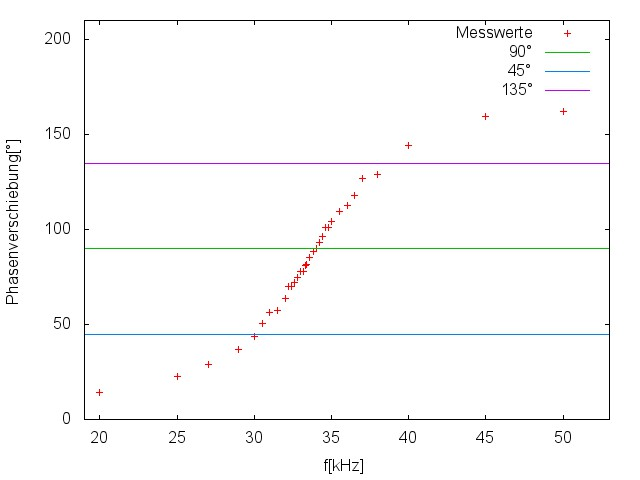
\includegraphics[width = 12cm]{img/graph_d.jpg}
		\caption{Phase der Spannung in Abh"angigkeit von der Freuquenz}
		\label{phase}
	\end{figure}

	\begin{table}
\begin{center}
\begin{tabular}{r|r|r|r|r|r|r|r|r|r|r|r|}
f[$\SI{}{\kilo\hertz}$] & a & b & a/b & f[$\SI{}{\kilo\hertz}$] & a & b & a/b & f[$\SI{}{\kilo\hertz}$] & a & b & a/b\\
\hline
1 & 0 & 4 & 0 & 30.5 & 0.9 & 6.4 & 0.141 & 33.2 & 2.6 & 12 & 0.216\\
5 & 0 & 8 & 0 & 31 & 1 & 6.4 & 0.156 & 33.3 & 2.7 & 12 & 0.225\\
10 & 0.1 & 10 & 0.01 & 31.5 & 2 & 12.6 & 0.159 & 33.4 & 2.7 & 11.9 & 0.227\\
15 & 0.2 & 6.8 & 0.029 & 32 & 2.2 & 12.4 & 0.177 & 33.6 & 2.8 & 11.8 & 0.237\\
20 & 0.4 & 10 & 0.04 & 32.2 & 2.4 & 12.4 & 0.194 & 33.8 & 2.9 & 11.8 & 0.246\\
25 & 0.5 & 8 & 0.063 & 32.4 & 2.4 & 12.4 & 0.194 & 34 & 2.9 & 11.6 & 0.25\\
27 & 0.6 & 7.4 & 0.081 & 32.6 & 2.4 & 12 & 0.2 & 34.2 & 3 & 11.6 & 0.259\\
29 & 0.7 & 6.8 & 0.103 & 32.8 & 2.5 & 12 & 0.208 & 34.4 & 3.1 & 11.6 & 0.267\\
30 & 0.8 & 6.6 & 0.121 & 33 & 2.6 & 12 & 0.216 & 34.6 & 3.2 & 11.4 & 0.281\\
\end{tabular}
\end{center}
\begin{center}
\begin{tabular}{r|r|r|r|r|r|r|r}
f[$\SI{}{\kilo\hertz}$] & a & b & a/b & f[$\SI{}{\kilo\hertz}$] & a & b & a/b \\
\hline
34.8 & 3.2 & 11.4 & 0.281 & 38 & 3.8 & 10.6 & 0.358 \\
35 & 3.3 & 11.4 & 0.289 & 40 & 4 & 10 & 0.4 \\
35.5 & 3.4 & 11.2 & 0.304 & 45 & 3.9 & 8.8 & 0.443 \\
36 & 3.5 & 11.2 & 0.313 & 50 & 3.6 & 8 & 0.45 \\
36.5 & 3.6 & 11 & 0.327 & 75 & 2.6 & 5.4 & 0.481 \\
37 & 3.8 & 10.8 & 0.352 & 100 & 2 & 4 & 0.5 \\
\end{tabular}
\caption[smallcaption]{longcaption}
\label{phase}
\end{center}
\end{table}
